\documentclass{article}
\usepackage[utf8]{inputenc}
\usepackage{multicol}
\usepackage{graphicx}
\usepackage[round]{natbib}
\usepackage{hyperref}
\usepackage{amsmath}
\usepackage{framed}
\usepackage{palatino}
\usepackage[absolute]{textpos}
\usepackage{xcolor}
\usepackage{setspace}
\usepackage{float}
\onehalfspacing

\begin{document}
\begin{titlepage}
\def\coverborderleft{30mm}
\definecolor{UniversitaetFarbe}{RGB}{0,101,189}

\begin{textblock*}{\textwidth}(\coverborderleft, 2cm)
\noindent
\textcolor{UniversitaetFarbe} {
  \fontsize{9}{11}\selectfont
  \sffamily Master of Science in Transportation Systems\\
  \sffamily Ingenieurfakultät Bau Geo Umwelt\\
  \sffamily Technische Universität München}
\end{textblock*}

\begin{textblock*}{19mm}[1,0](19cm, 2cm)
  
\includegraphics{TUM_blau.pdf}
\end{textblock*}

\begin{textblock*}{\paperwidth}(\coverborderleft, 6cm)
\raggedright
  \sffamily \huge{The Feedback Loop of Cycling and Walking} \\
  \sffamily \Large{David Bailey (david.bailey@tum.de) | 03682683}\\
  \sffamily \large{February 2017}\\
\end{textblock*}
~\\
\end{titlepage}

\tableofcontents
\newpage

\section{Abstract}
\subsection*{Objective}
Deutsche Bahn, the primary owner and operator of the German railway network, provides popular passenger service across the country. However, the company suffers from low customer satisfaction scores and poor punctuality. This paper seeks to explore how Deutsche Bahn can improve customer satisfaction, ridership, and revenue by implementing a customer-focused culture. 
\subsection*{Methods}
First, we examine how a customer-focused organization operates and what service quality is. Then we evaluate the areas where Deutsche Bahn is customer-focused and where they can improve. 
\subsection*{Results}
We present several opportunities for implementing a customer-focused culture at Deutsche Bahn. These changes should enhance service quality and customer satisfaction though improvements to ticketing, travel time, punctuality, and transparency. Examples are provides of successful programs from railways in neighboring countries including Austrian Federal Railways (ÖBB), Dutch Railways (NS), and Swiss Federal Railways (SFF CFF FFS). However these companies all operate much smaller networks than Deutsche Bahn.
\subsection*{Discussion}
Deutsche Bahn often chooses engineering solutions to its customer service problems. Additionally, because the Federal Republic of Germany is the sole owner of Deutsche Bahn, the organization often operates more as a political entity that a service company. However, the changing landscape of transportation in Europe will soon force Deutsche Bahn to adapt or decline.
\subsection*{Conclusions}
To increase ridership and remain competitive with car and air transportation, Deutsche Bahn must work to implement a customer-focused culture.
\newpage
\section{Introduction}
The first steam powered railway in Germany opened in Bavaria on December, 7th 1835 carrying passengers between Fürth and Nürnberg. Over the last two centuries, the German railway network has grown into one of the largest and most complex networks in the world. Deutsche Bahn AG, a private company owned by the Federal Republic of Germany, owns most of Germany's railway infrastructure through the subsidiary DB Netze and operates most of Germany's passenger trains through the subsidiaries DB Fernverkehr and DB Regio. (Deutsche Bahn also owns DB Schenker, a logistics subsidiary, and several foreign transportation subsidiaries.) A summary of the services operated by Deutsche Bahn is provided in Table \ref{table:services}.

\begin{table}[H]
  \centering
\begin{tabular}{ l | l }
International/National (DB Fernverkehr) & Regional (DB Nahverkehr) \\
\hline
Intercity-Express (ICE) & Interregio-Express (IRE) \\
InterCity (IC) & Regional Express (RE) \\
EuroCity (EC) & Regionalbahn (RB) \\
 & S-Bahn (S)\\
\end{tabular}
    \caption{Deutsche Bahn Services \citep{db}}
    \label{table:services}
\end{table}

In 2015, German railways carried 2.708 billion passengers (21.9\% of all passengers carried, excluding private cars) and 367,314,000 tonnes of goods (8.1\% of all goods) along along a network that measured 37,775 km in 2014 (Figure \ref{fig:comparison}) \citep{destatis}. When compared with road transportation, railways carry significantly more passengers per kilometer of network length.

\begin{figure}[H]
    \centering
    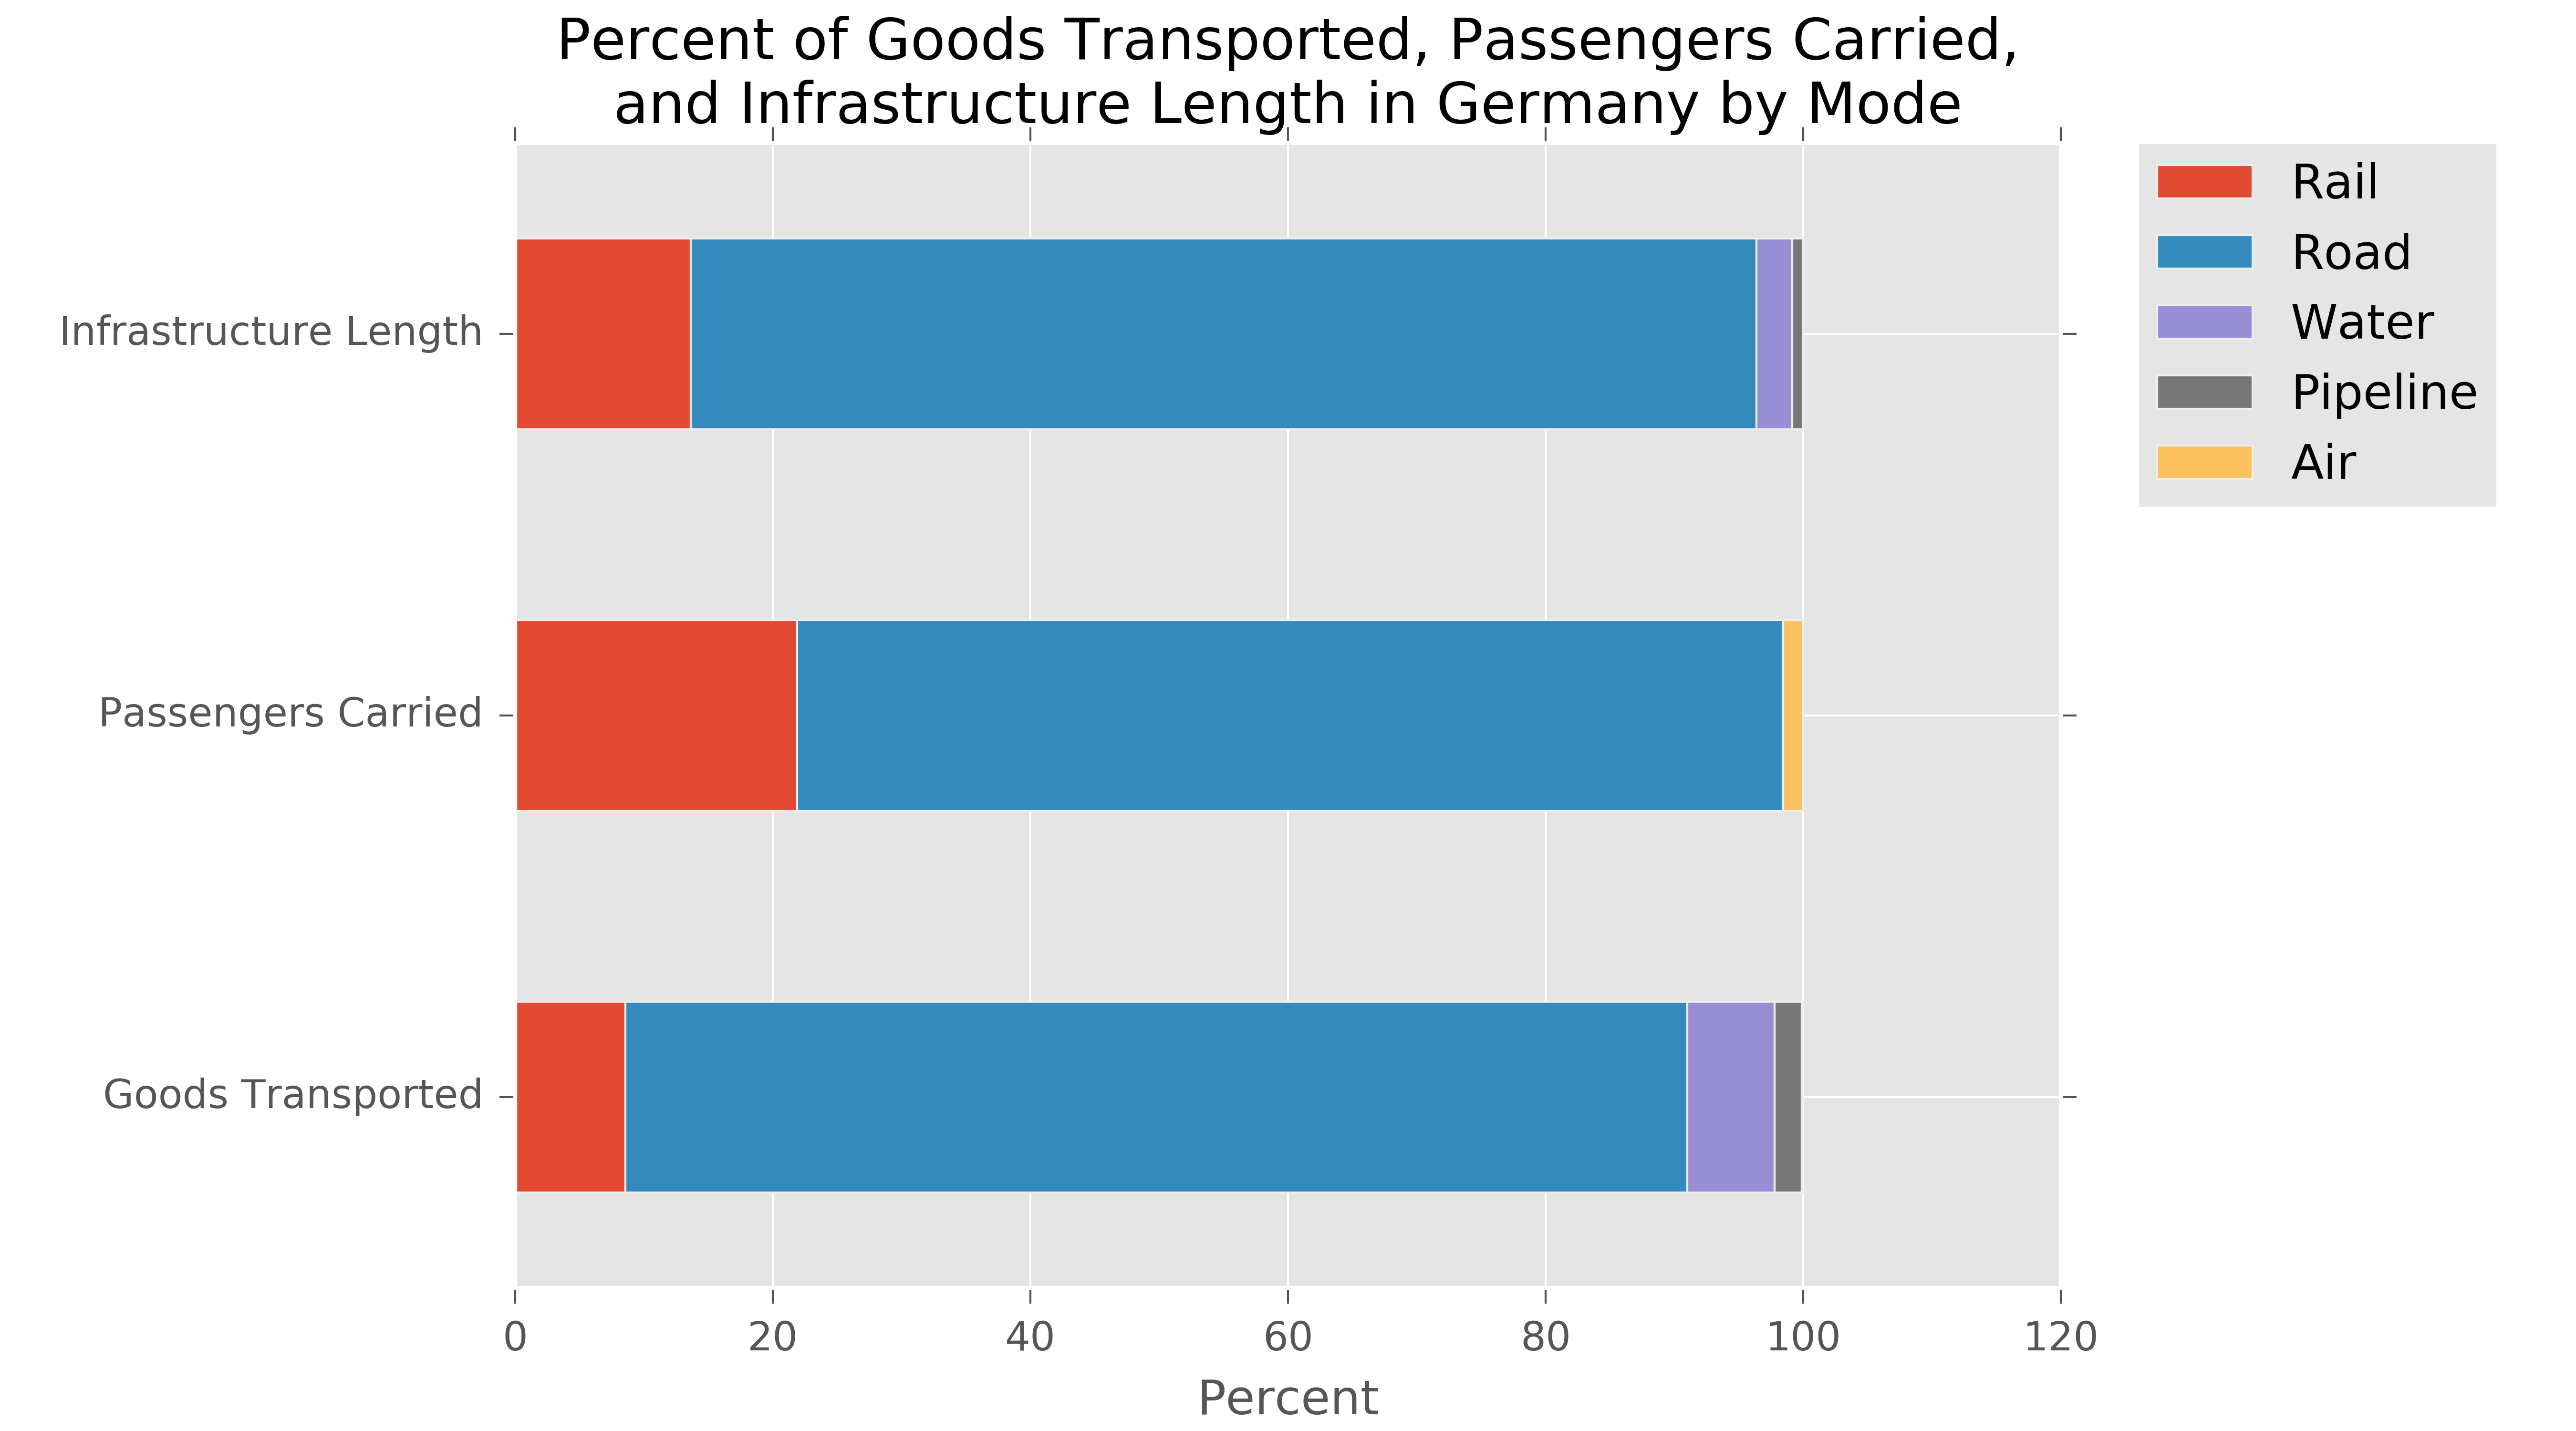
\includegraphics[width=\textwidth]{comparison.png}
    \caption{Percent of Goods Transported, Passengers Carried, and Infrastructure Length in Germany by Mode (2015) \citep{destatis}}
    \label{fig:comparison}
\end{figure}

As shown in Table \ref{table:modeshare}, rail is often the preferred mode for long distance trips, especially business trips in Germany \citep[Page 97]{reichert2015}. While mode choice for urban trips is often determined mostly by travel time, long distance travel travelers also tend to consider the cost and comfort of different modes \citep[Page 8-12]{moeckel2015}. Additionally, although long distance trips are far less common than urban trips, they account for a disproportionately large number of kilometers traveled and therefore can create disproportionately larger social and environmental effects.

\begin{table}[H]
  \centering
\begin{tabular}{ l | r r r r }
    Mode & Car & Train & Air & Other \\
    \hline
    Private & 64.1\% & 14.9\% & 12.9\% & 8.1\% \\
    Business & 52.6\% & 22.9\% & 21.7\% & 2.8\% \\
    Total & 61.9\% & 16.4\% & 14.6\% & 7.1\% \\
\end{tabular}
    \caption{Mode Share of Long Distance Trips in Germany (2008) \citep[Page 97]{reichert2015}}
    \label{table:modeshare}
\end{table}

However, even though the railway network enjoys a large share of passenger transportation, Deutsche Bahn's customer satisfaction scores (Table \ref{table:customerservice}) and punctuality (a component of customer satisfaction) (Table \ref{table:punctuality}) are relatively low \citep{db2016}. This paper seeks to explore how Deutsche Bahn can implement a customer-focused culture improving customer satisfaction and consequently ridership and revenue. 

\begin{table}[H]
  \centering
\begin{tabular}{ l | r | r | r }
 & 2013 & 2014 & 2015 \\
\hline
DB Fernverkehr & 74 & 75 & 75 \\
DB Regio & 68 & 69 & 71 \\
\end{tabular}
    \caption{Customer Satisfaction \citep{db2016}}
    \label{table:customerservice}
\end{table}

\begin{table}[H]
  \centering
\begin{tabular}{ l | r | r | r }
 & 2013 & 2014 & 2015 \\
\hline
DB Fernverkehr & 94.1\ & 94.5 & 93.7 \\
DB Regio & 73.9 & 76.5 & 74.4 \\
\end{tabular}
    \caption{Punctuality (\%) \citep{db2016}}
    \label{table:punctuality}
\end{table}

Before the invention of the automobile and the airplane, railways had a monopoly on motorized transportation. However, today, cars are a very competitive mode for short and medium distances and planes are much faster for traveling long distances \citep[Page 2]{laube2008}. Therefore, rail must compete with fast and reliable travel times and high levels of comfort.

\section{Methods}
First, we examine how a customer-focused organization operates and what service quality is. Then we evaluate the areas where Deutsche Bahn is customer-focused and where they can improve. Comparisons with neighboring countries (Austrian Federal Railways (ÖBB), Dutch Railways (NS), and Swiss Federal Railways (SFF CFF FFS)) are provided. However these companies all operate much smaller networks than Deutsche Bahn.

\section{Results}
\subsection{Customer-focused Organizations}
In a customer-focused organization, the organization's goal should match its customers' goal. For Deutsche Bahn, its goal should be its customers' travel goal. Historically, railways, including Deutsche Bahn, have focused on transporting the maximum amount of passengers while keeping costs low. However, this goal often does not align with an individual's goal of getting from point a to point b, quickly, reliably, comfortably, and for a good price. This gap between what the customer desires and what the service provider provides has caused a lack of confidence and trust in Deutsche Bahn and other railways.

\subsection{Service Quality}
Service Quality, as defined in EN 13816 "Public transport services; Definition, definition of performance targets and measurement of service quality", is a measure of the difference between what the customer expects and what the service provider delivers. As described in Figure \ref{fig:servicequality}, the difference between the customer's expectations and perception determines his satisfaction, and the difference between the service provider's planned and delivered service quality determines its performance. Additionally, EN 13816 provides a uniform way to measure service quality \citep{en13816}. 

\begin{figure}[H]
    \centering
    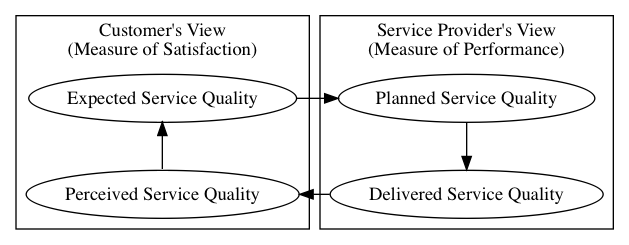
\includegraphics[width=\textwidth]{din.png}
    \caption{The System of Service Quality \citep{en13816}}
    \label{fig:servicequality}
\end{figure}

\subsection{Customer Satisfaction}
Providing high service quality in a customer-focused organization means putting the customer's needs first. The Netherlands accomplishes this by setting targets for Dutch Railways. If Dutch Railways, the service provider, misses a performance target, they must pay a fine \citep{ns-transparent}. However, with the low customer satisfaction scores shown in Table \ref{table:customerservice}, it appears there is no penalty for Dutsche Bahn.

\begin{framed}
\noindent A pretty cool thing about the Dutch Railways is that one of our biggest targets, and a main driver as a whole, is our customer satisfaction score. --Fokko van der Schans, Dutch Railways \citep{lawson2017}
\end{framed}

\subsection{Ticketing}
Ticketing is an area where Deutsche Bahn is already customer-focused. They offer several options: Flexpreis (flexible tickets), Sparpreis (cheap tickets), and group tickets (e.g. Bayern Ticket). They also have a frequent travel card, Bahn Card, and children under 15 travel free with an adult. However, although Deutsche Bahn offers mobile tickets on the DB Navigator app, but they do not offer a country-wide electronic ticketing card like Dutch Railways' OV-chipkaart.

\subsection{Travel Time}
Swiss Federal Railways implemented the Bahn 2000 program to increase frequencies and create a clock-face schedule. While these objectives necessitated an increase in speed on some routes, the primary goal of the project was not decreasing travel times though faster trains, but more frequency and better connections \citep[Page 5]{laube2008}. Dutch Railways has also increased frequency and implemented clock-face scheduling in recent years. This has also enabled them to change many integrated lines to independent lines so delays from one line do not propagate to other lines \citep{ns-railway}. These changes have resulted in a positive response from customers. Austrian Federal Railways has also implemented clock-face scheduling. Operating a clock-face schedule, which Deutsche Bahn is working towards, still leaves the network vulnerable to service disruptions. However, by also the increasing frequency of service, passengers who miss a connection because of delays have a higher probability of catching another train sooner.

\subsection{Punctuality}
Unlike air and road transportation, railways are in control of the level of congestion on their infrastructure which should allow for high punctuality (reliable travel times). This is a tremendous advantage over other modes that should lead to high customer satisfaction. However, if a railway experiences low punctuality, they miss out on this advantage.

Punctuality, is easy to measure, but often hard to communicate with customers. First, the service provider and customer must agree on how of a delay is acceptable. The typically accepted value is five minutes, but five minutes could be the difference between making a connection and waiting for the next train. Second, they must agree on how to count delays. There are two prominent methods: the percentage of late trains and the percentage of late stops.

\begin{align}
\frac{Number\ of\ trains\ that\ service\ all\ stops\ within\ the\ delay\ threshold}{Total\ number\ of\ trains\ operated\ in\ a\ year}
\end{align}

\begin{align}
\frac{Number\ of\ stops\ serviced\ within\ the\ delay\ threshold}{Total\ number\ of\ stops\ serviced\ in\ a\ year}
\end{align}

Obviously the second method usually gives higher percentages for busy railways because one late stop does not penalize the entire train. However, if that one stop is where the majority of passengers alight, the percentage may not be a truthful representation of the magnitude of delays. The is the method Deutsche Bahn uses, and they set a acceptable amount of delay time at six minutes because of software issues. Deutsche Bahn's punctuality percentages are shown in Table \ref{table:punctuality} in the introduction. Deutsche Bahn often blames construction for delays, but a 2013 analysis of Deutsche Bahn's own data shows that construction is indicated as the reason for only 9\% of delays \citep{w2013}.

As a comparison with neighboring operators, for Dutch Railways, in November 2016, 89.5\% of all trains arrived within 5 minutes of the scheduled arrival time \citep{ns-howmany}. However, their agreement with the government is that 93\% of trains will arrive within 5 minutes of the scheduled arrival time. For Austrian Federal Railways, in 2016, 86.7\% of long distance trains, 96.4\% of regional trains, and 95.9\% of all trains arrived with 5 minutes of the scheduled arrival time \citep{oebb}. Punctuality is an area where Deutsche Bahn could greatly improve service quality.
\subsection{Transparency}
Put simply, Deutsche Bahn is lacking in transparency. Its customers know there are problems with service, but instead of admitting to the problems and providing honest reasons and solutions, Deutsche Bahn often provides no information. For example, Dutch Railways provides punctuality information for all routes to customers at the point of sale. Deutsche Bahn used to have an publicly-available interface for querying punctuality information and the reasons for delays. However, they disabled this interface in 2013 \citep{w2013}. Recently, Deutsche Bahn launched an open data platform, data.deutschebahn.com, but the service only provides limited data about schedule information and related services. For Deutsche Bahn to align with its customers, it must first be transparent with them.

\section{Discussion}
Deutsche Bahn often chooses engineering solutions to its customer service problems. Examples of this include spending tremendous sums of money to construct new high-speed lines (e.g. Munich to Berlin) and rebuilding old train stations (e.g. Berlin, Stuttgart). Deutsche Bahn often claims these projects are necessary to improve service, but critics contest that increasing frequency and/or better coordination of services are cheaper and better options. Deutsche Bahn's ex-CEO Rüdiger Grube's newest improvement program, Railway of the Future (Zukunft Bahn), again tries to solve the company's customer satisfaction problem with more technology (WiFi, mobile apps), new trains, and "specialist teams to improve the punctuality of trains" \citep{db-programm}. While the program claims to be customer-focused, which is a good first step, it fails to address Deutsche Bahn's lack of alignment with its customers' travel goals the way the Austrian, Dutch, and Swiss railways have over the past decades. As mentioned in the introduction, Deutsche Bahn operates a much larger and more complex network than its neighbors. However, Detusche Bahn appears ignorant to their successful efforts and is insistent that somehow "business as usual" will have better than usual results.

Although this article has focused on Deutsche Bahn's passenger services, the company should also improve the customer focus of the freight business. With the European Union's Shift2Rail initiative promoting a shift from road modes to rail modes, Deutsche Bahn has a great business opportunity to grow its freight business \citep{shift2rail}. Additionally, while the company positions itself as a green transportation company, its focus on passenger transportation means the vast majority of goods movement in Germany is done so with trucks as shown in Figure \ref{fig:comparison}. By shifting more freight from road to rail, Deutsche Bahn could reduce pollution and help Germany meet its climate goals.

With the Federal Republic of Germany as the sole owner of Deutsche Bahn, the organization often operates more as a government entity than a private company. Historically, the government has protected the organization though laws such as a ban on long distance bus transportation from 1931 to 2011. Also, a ban on night flights in the country, while officially to limit noise pollution, is also beneficial for Deutsche Bahn. However, the political landscape in Europe is changing: European Union regulations require strict separation between rail infrastructure owners and rail service operators. Deutsche Bahn met these requirements by creating separate subsidiaries with different responsibilities, although many claim their current scheme violates the regulations. Nevertheless, the writing is on the wall that European rail operators must adapt their business models from functioning as government entities to free market competitors. Consequently, the federal government should impose strict and transparent requirements on Deutsche Bahn regarding customer satisfaction and punctuality with appropriate penalties for failure to meet the requirements. Currently, there are strong regulations regarding the technical construction and operation of railways, but weak controls regarding service quality. Unfortunately, the main feedback mechanism is currently public dissatisfaction and consequently political pressure which to which Deutsche Bahn often deflects the blame for their lack of service to circumstances outside their control.

\section{Conclusion}
Deutsche Bahn operates a highly complex rail network with limited resources. Shifting towards a customer-focused culture will allow the company to improve customer satisfaction, grow ridership, and increase revenues. To improve as a service provider, Deutsche Bahn must align its goals with its customers' travel goals.
\bibliographystyle{plainnat}
\bibliography{references}
\end{document}